\documentclass[10pt,twocolumn,letterpaper]{article}

\usepackage[review]{cvpr}
%% This file contains a number of tweaks that are typically applied to the main document.
%% They are not enabled by default, but can be enabled by uncommenting the relevant lines.


%%
%% Official support for 2-column teaser figure
%%
\usepackage{cuted} %< for strip environment

%%
%% For auto-referencing of figures (see fig/teaser.tex and \label{} therein) 
%%
\usepackage{currfile} %< for \currfilebase macro

%%
%% caption and (global) spacing overrides
%%
\usepackage{caption} %< for "\captionof" commands (teaser)
% \setlength{\abovecaptionskip}{.5em} % space above caption
% \setlength{\belowcaptionskip}{1em} % space below caption

%%
%% Inline annotations; for predefined colors, refer to "dvipsnames" in the xcolor package:
%% https://tinyurl.com/overleaf-colors
%%
\newcommand{\red}[1]{{\color{red}#1}}
\newcommand{\todo}[1]{{\color{red}#1}}
\newcommand{\TODO}[1]{\textbf{\color{red}[TODO: #1]}}
%%
%% Disable for camera ready / submission by uncommenting these lines:
%%
% \renewcommand{\TODO}[1]{}
% \renewcommand{\todo}[1]{#1}

%%
%% Work harder in optimizing text layout. Typically shrinks text by 1/6 of page, enable
%% it at the very end of the writing process, when you are just above the page limit.
%%
% \usepackage{microtype}

%%
%% Fine-tune paragraph spacing.
%%
% \renewcommand{\paragraph}[1]{\vspace{.5em}\noindent\textbf{#1.}}

%%
%% Globally adjusts space between figure and caption.
%%
% \setlength{\abovecaptionskip}{.5em}

%%
%% Allows "the use of \paper to refer to the project name"
%% with automatic management of space at the end of the word.
%%
% \usepackage{xspace}
% \newcommand{\paper}{ProjectName\xspace}

%%
%% Commonly used math definitions.
%%
% \DeclareMathOperator*{\argmin}{arg\,min}
% \DeclareMathOperator*{\argmax}{arg\,max}

%%
%% Tighten underline.
%%
% \usepackage{soul}
% \setuldepth{foobar}

%%
%% Reconfigure paragraph (tweaks spacing)
%%


\definecolor{cvprblue}{rgb}{0.21,0.49,0.74}
\usepackage[pagebackref,breaklinks,colorlinks,allcolors=cvprblue]{hyperref}

\def\paperID{3201}
\def\confName{CVPR}
\def\confYear{2026}

\title{Video Super-Resolution with Temporal Consistency\\
on REDS4 and Vid4}

\author{Yuming Zhang\\
The Hong Kong University of Science and Technology (Guangzhou)\\
Student ID 50025933\\
{\tt\small yzhang395@connect.hkust-gz.edu.cn}
\and
Jiayang Liu\\
The Hong Kong University of Science and Technology (Guangzhou)\\
Student ID 50027216
}

\begin{document}
\maketitle

\begin{abstract}
Given a low-resolution video, we reconstruct a high-resolution video that recovers spatial detail and stays stable across frames.
The shared input is the official $4\times$ bicubic release, not a downsample recomputed by our own kernel.
Part~1 compares bicubic and Lanczos upsampling, a frame-wise EDSR baseline, and a course temporal average.
Part~2 runs EDVR and records the released TecoGAN checkpoint as a TensorFlow model that this Python environment cannot load.
Part~3 treats Pyramid Flow as a conditioned generator only when the sampler can start from a noisy bicubic upsample, runs STAR from its released weights, and blends BasicVSR++ with STAR through a disagreement map.
REDS4 is scored on RGB with no border crop.
The extra benchmark is Vid4, with the official BasicSR $4\times$ bicubic frames. The MIT Vimeo test archive returns HTTP 403, so that 30-clip subset is not scored.
The public repository is \url{https://github.com/Oliver-ming/Intro_to_CV_project_1}.
\end{abstract}

\section{Introduction}
Video super-resolution maps a low-resolution sequence to a high-resolution sequence.
Doing this frame by frame can raise pixel scores while the restored detail flickers.
The course task therefore asks for both spatial detail and temporal consistency.

We follow one comparison protocol.
Every method sees the same official $4\times$ bicubic low-resolution frames~\cite{nah2019reds,xue2019vimeo}.
A model trained on a different degradation is still run on that input, and the table names its training degradation.
We do not pretrain Pyramid Flow or STAR.
Where the assignment asks for an exploration that the released code does not support, we keep the attempt and write the failure instead of substituting an unrelated sample.

\section{Related Work}
Single-image networks learn a mapping from a low-resolution patch to a high-resolution patch.
SRCNN introduced a convolutional mapping~\cite{dong2015srcnn}.
EDSR deepened residual blocks for bicubic super-resolution~\cite{lim2017edsr}.
SRGAN traded distortion for sharper textures with an adversarial loss~\cite{ledig2017srgan}.
These models do not look at neighboring frames.

Video methods add alignment and fusion.
EDVR aligns a short window with pyramid cascading deformable convolution and fuses it with temporal-spatial attention~\cite{wang2019edvr}.
TDAN also aligns with deformable convolution over time~\cite{tian2020tdan}.
BasicVSR argued that bidirectional propagation, feature alignment, and pixel-shuffle upsampling are the essential pieces~\cite{chan2021basicvsr}.
BasicVSR++ adds second-order grid propagation and flow-guided deformable alignment~\cite{chan2022basicvsrpp}.

Generative video models push the other side of the distortion--perception trade-off.
TecoGAN uses a recurrent generator, a spatio-temporal discriminator, and a temporal loss, and it measures temporal change with tLP~\cite{chu2020tecogan}.
Flow matching learns a vector field from noise to data~\cite{lipman2023flow}.
Pyramid Flow applies that idea in a pyramid for text-to-video and image-to-video generation~\cite{jin2025pyramid}; it is not a published super-resolution model.
STAR adapts a text-to-video backbone with ControlNet and a local insertion module for real-world video super-resolution~\cite{xie2025star}.
LoRA is a low-rank update used as a course experiment here, not as STAR's training recipe~\cite{hu2022lora}.

Quality is not one number.
SSIM compares structure~\cite{wang2004ssim}.
LPIPS compares deep features~\cite{zhang2018lpips}.
REDS, Vid4, and Vimeo-90K are the usual bicubic video super-resolution benchmarks~\cite{nah2019reds,xue2019vimeo}.
This report scores REDS4 and Vid4.

\section{Method}
\subsection{Shared input}
REDS4 is clips 000, 011, 015, and 020, held out from the REDS training split.
Low-resolution frames come from \texttt{train\_sharp\_bicubic/X4}, the MATLAB \texttt{imresize} bicubic track used by EDVR and BasicVSR.
Our bicubic and Lanczos kernels only upsample those frames.
They are checked against OpenCV and are not used to rebuild the benchmark input.

Vid4 is calendar, city, foliage, and walk, taken from BasicSR's public Vid4 archive.
Low-resolution frames are the official \texttt{BIx4} track, and ground truth is the \texttt{GT} track in the same archive.
This is not Vimeo-90K.
The frozen 30-clip Vimeo list remains in \texttt{docs/manifests/vimeo-subset.txt}, and it is not scored: both MIT test archives return HTTP 403.

\subsection{Part 1}
Bicubic upsampling uses OpenCV's cubic ($a=-0.75$), four taps, and replicated borders.
Lanczos uses radius 4, eight taps, and renormalized weights.
Both map output pixel $i$ to source coordinate $(i+0.5)/\mathrm{scale}-0.5$.
EDSR is the official baseline with 16 residual blocks and 64 features, loaded from the DIV2K $4\times$ checkpoint and not trained here~\cite{lim2017edsr}.

The temporal average is a course binomial smoother, not a kernel from those papers.
After bicubic upsampling, each frame is averaged with two neighbors on either side using weights $[1,4,6,4,1]/16$.
Weights that fall off the clip are dropped and the rest are renormalized.
Unsharp masking is an extra variant of that average,
$y = x + 1.0\,(x - G_{\sigma=1}(x))$,
then clamped to the valid range.
Sigma 1 and amount 1 are course defaults.

\subsection{Part 2}
EDVR-L uses the released bicubic checkpoint through BasicSR: 128 features, five input frames, deformable groups 8, TSA fusion, and \texttt{reflection\_circle} padding~\cite{wang2019edvr}.
On a 100-frame clip the window for the first frame is indices 4, 3, 0, 1, 2.
The REDS blur-downsampling checkpoint is not this row.
The 7-frame Vimeo-90K EDVR-L checkpoint is a different file and is not loaded into this 5-frame model. Vid4 uses the same REDS bicubic checkpoint as REDS4.

The released TecoGAN archive is a TensorFlow~1 checkpoint~\cite{chu2020tecogan}.
\texttt{env\_cv} is Python~3.10 and cannot install TensorFlow~1, so those weights are not loaded.
A later PyTorch $4\times$ checkpoint, if one runs, is reported separately and is not called the released model.

\subsection{Part 3}
Pyramid Flow's released model generates video from text, and its image-to-video path animates a clean first frame~\cite{jin2025pyramid}.
A result enters the metric table only when the official sampler can noise the whole bicubic-upscaled clip and integrate from a start near the middle of its own schedule.
The table records that start index and the number of function evaluations.
Official image-to-video and pure text-to-video samples do not.
The pinned Pyramid Flow source (\texttt{a012faa1}) exposes only those two entry points, so the official interface stays a failure case in \texttt{docs/results/pyramid\_flow\_attempt.json}.
A separate course sampler encodes the bicubic upsample with the released VAE, mixes noise at the middle index of the last-stage schedule, and continues with \texttt{scheduler.step}.
On REDS4 that sample starts at index 10 of 20 last-stage steps and scores 17.94\,dB.
It is not the released \texttt{generate()} path.

STAR's official row is inference with the released weights on the shared bicubic input.
Its training degradation is real-world (OpenVid with a Real-ESRGAN-style pipeline), and the table says so~\cite{xie2025star}.
A second row is a course LoRA experiment: rank 8, 200 steps, batch size 1, learning rate $10^{-4}$, on 20 Vimeo-90K training septuplets that are not in the test subset~\cite{hu2022lora}.
Only injected LoRA weights are trained.
The row is judged by whether tLPIPS drops.
If the released code has no LoRA interface, the row is a failure case.
Pinned STAR \texttt{69b8bc53} trains ControlNet and parameters named \texttt{local}, not LoRA, so that row is the failure recorded in \texttt{docs/results/star\_lora\_attempt.json}.
The released light-degradation checkpoint is the official inference row. Its download is separate from the LoRA failure.
The released U-Net calls \texttt{xformers} attention, and that package is pinned to an older PyTorch.
This run keeps torch~2.11 and uses scaled dot-product attention for the same bias-free call.

The hybrid does not train a router.
BasicVSR++ supplies the fidelity frame when a $4\times$ bicubic checkpoint matched to the benchmark is available~\cite{chan2022basicvsrpp}.
The generative frame is official STAR inference.
Face and text boxes come from OpenCV \texttt{FaceDetectorYN} (YuNet) and \texttt{TextDetectionModel\_EAST}, run on the bicubic-upscaled frame, with no dilation.
Those detectors are course tools.
Pixels inside the boxes are taken from BasicVSR++.
Elsewhere the blend weight is the per-frame min--max normalized mean absolute RGB difference between the fidelity frame $f$ and the generative frame $g$,
\begin{equation}
w = \mathrm{norm}\!\left(\frac{1}{3}\sum_{c=1}^{3}|f_c-g_c|\right),
\end{equation}
and the restored frame is $(1-w)f + wg$.
Certain pixels set $w=0$.
There is no Gaussian smoothing and no extra global weight.
This disagreement map is not a published uncertainty estimator.
If STAR does not run, the hybrid is a failure case.

\section{Experiments}
\subsection{Clip geometry}
Each REDS4 clip has 100 frames.
The official low-resolution frames are $180\times320$, and the ground-truth frames are $720\times1280$, so the shared scale is exactly 4.
Four clips give 400 frames.
Vid4 has 171 frames: calendar 41, city 34, foliage 49, and walk 47.
Ground-truth sizes are $720\times576$, $704\times576$, $720\times480$, and $720\times480$.
The low-resolution frames are exactly one quarter of those sizes.
Full-reference scores use every frame.
There is no border crop and no held-out frame inside a clip.

\subsection{Protocol}
PSNR and SSIM~\cite{wang2004ssim} on REDS4 and on Vid4 use RGB and no border crop, including every frame.
LPIPS uses AlexNet on RGB~\cite{zhang2018lpips}.
tLPIPS is TecoGAN's tLP~\cite{chu2020tecogan}.
With $d$ the AlexNet LPIPS of two frames,
\begin{equation}
\mathrm{tLPIPS} = \frac{1}{T-1}\sum_{t=2}^{T}\bigl|d(\hat{x}_t,\hat{x}_{t-1}) - d(x_t,x_{t-1})\bigr|.
\end{equation}
We report that value, not the $\times 100$ display scale used in the paper's tables.
FID pools the restored frames against the ground-truth frames of that set.
The report states the frame count, so the number is not compared with a full-dataset paper FID.
Scores use 8-bit quantized frames.
Full-reference scores require ground truth.
A filmed clip has no ground-truth video, so it is judged visually and is not entered in the score tables.

\subsection{Filmed clips}
Four clips were filmed at \(1920\times1080\): a person beside a poster (161 frames), shrubs (146), a pond (290), and a dark classroom (259).
Official STAR does not fit a \(1920\times1080\) frame in 24\,GB, so each frame is area-resized to \(1280\times720\) and then downsampled with OpenCV's \(4\times\) bicubic kernel.
That low-resolution input is not an official benchmark release.
The same REDS bicubic checkpoints used on REDS4 restore these frames.
Figure~\ref{fig:wild} is frame 80 of the poster clip.
Bicubic upsampling leaves the glasses and the poster text soft.
EDVR-L draws those edges closer to the filmed frame.
In this crop, BasicVSR++ carries the vertical slats onto the face.
That is this checkpoint on a filmed scene, not a REDS4 score.

\begin{figure}[t]
\centering
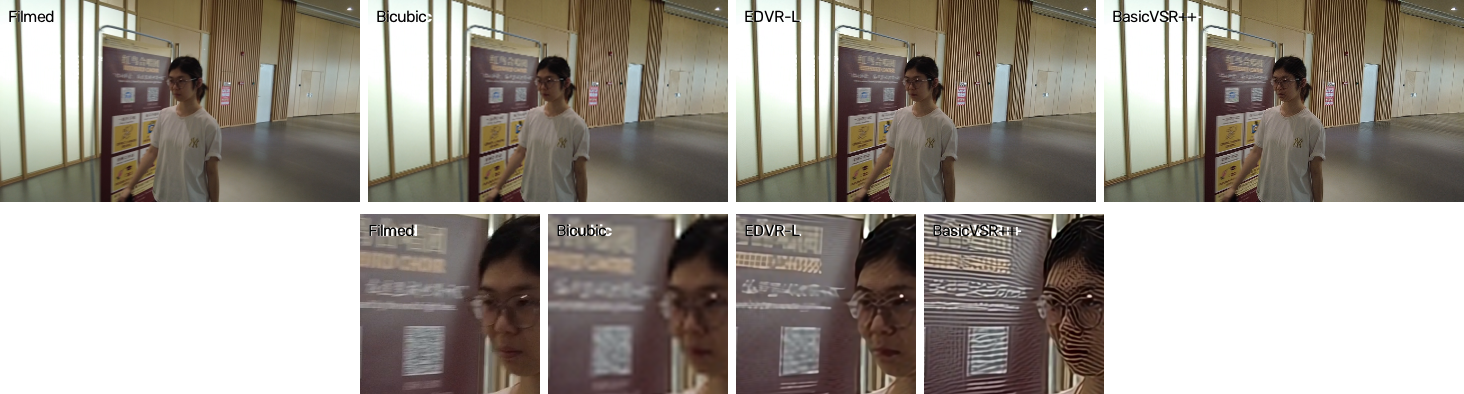
\includegraphics[width=\linewidth]{figures/wild_face_text.png}
\caption{Filmed poster clip, frame 80. Top: the \(1280\times720\) filmed frame, bicubic upsampling, EDVR-L, and BasicVSR++. Bottom: one \(180\times180\) crop on the poster text and the glasses. There is no ground truth, so this figure is not scored.}
\label{fig:wild}
\end{figure}

\subsection{What has been run}
Table~\ref{tab:status} records the state of each row. Every REDS4 method that ran has 100 frames in each of clips 000, 011, 015, and 020, and Table~\ref{tab:metrics} gives the 400-frame scores. Vid4 uses the same checkpoints on the official \texttt{BIx4} frames, and Table~\ref{tab:vid4} gives those scores. The 7-frame Vimeo EDVR-L checkpoint is on disk and is not loaded into the 5-frame REDS model.

\begin{table}[t]
\centering
\caption{REDS4 rows on the shared official $4\times$ bicubic input. A failure is a missing interface, not a skipped direction.}
\label{tab:status}
\small
\begin{tabular}{@{}p{0.46\linewidth}p{0.48\linewidth}@{}}
\hline
Row & State \\
\hline
Bicubic, Lanczos & Scored \\
EDSR baseline, DIV2K $4\times$ & Scored, not trained \\
Temporal average, unsharp & Scored, course kernels \\
EDVR-L REDS bicubic & Scored \\
TecoGAN released & Failure: TensorFlow~1 checkpoint \\
TecoGAN PyTorch substitute & Scored, not the release \\
BasicVSR++ REDS4 bicubic & Scored \\
Pyramid Flow midpoint & Course sampler; official \texttt{generate()} unused \\
STAR light degradation & Four clips, one frame at a time \\
STAR course LoRA & Failure: no LoRA parameters \\
Disagreement-map hybrid & Blended and scored \\
Texture hybrid & Grass and water use STAR \\
\hline
\end{tabular}
\end{table}

BasicVSR++ uses the released REDS4 bicubic checkpoint with 64 mid channels and 7 residual blocks~\cite{chan2022basicvsrpp}.
The four clips are restored from \texttt{train\_sharp\_bicubic/X4}.
YuNet and the EAST text graph are both on disk. An empty detector mask does not by itself fail the blend.

\begin{figure}[t]
\centering
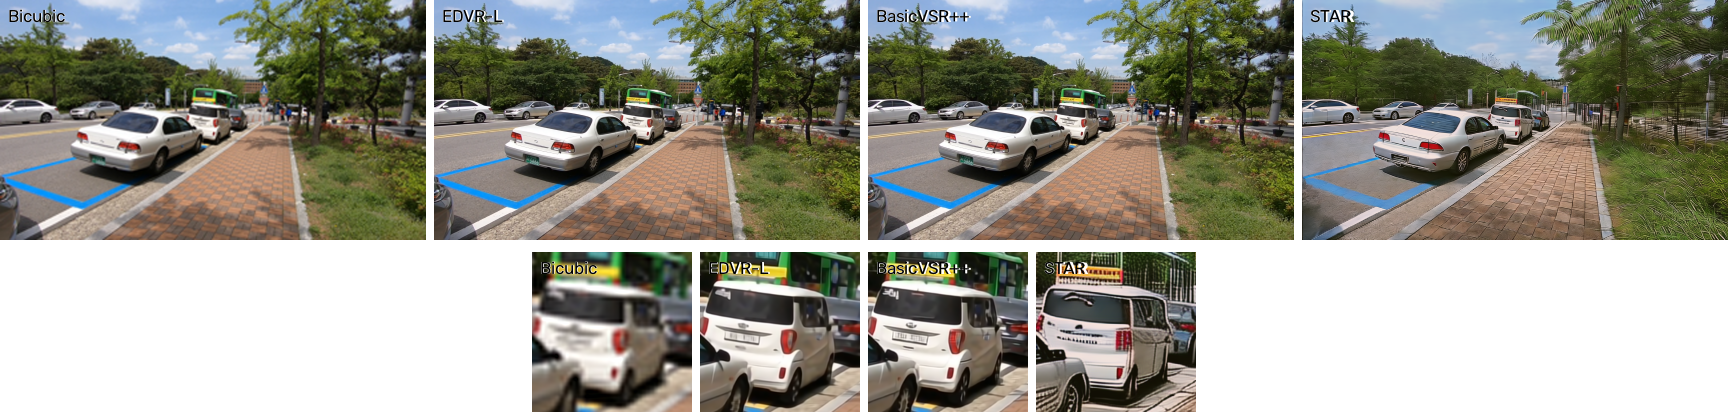
\includegraphics[width=\linewidth]{figures/reds4_000_frame050.png}
\caption{Clip 000, frame 50. Top: bicubic, EDVR-L, BasicVSR++, and official STAR. Bottom: the 160$\times$160 patch with the strongest bicubic detail. In that patch the car edges are softer after bicubic upsampling than after EDVR-L or BasicVSR++. STAR was trained on real-world degradation, so this bicubic input is outside that training degradation.}
\label{fig:reds-visual}
\end{figure}
The released TecoGAN weights and the STAR LoRA row stay failure cases.
Pyramid Flow's released \texttt{generate()} and \texttt{generate\_i2v} stay failure cases.
The course midpoint sampler is a separate row in Table~\ref{tab:metrics}: index 10 of 20 steps, 17.94\,dB, FID 165.99.
STAR and the non-official PyTorch TecoGAN are scored on the shared bicubic input and labeled as a mismatched degradation and a substitute checkpoint.
The released TecoGAN checkpoint has no score.

Table~\ref{tab:metrics} is the REDS4 score sheet.
Scores use 8-bit quantized frames.
The non-official TecoGAN row is listed so it cannot be confused with the released checkpoint.

\begin{table}[t]
\centering
\caption{REDS4 full-reference scores. PSNR, SSIM, LPIPS, and tLPIPS are averaged over clips 000, 011, 015, and 020. PSNR and SSIM are RGB with no border crop. tLPIPS is not scaled by 100. FID is one Fréchet distance on all 400 frames. Blank cells are not zeros.}
\label{tab:metrics}
\scriptsize
\resizebox{\linewidth}{!}{%
\begin{tabular}{@{}lccccc@{}}
\hline
Method & PSNR & SSIM & LPIPS & tLPIPS & FID \\
\hline
Bicubic & 26.24 & 0.7319 & 0.4577 & 0.0221 & 42.79 \\
Lanczos & 26.37 & 0.7365 & 0.4600 & 0.0229 & 36.74 \\
EDSR & 28.38 & 0.8077 & 0.2724 & 0.0042 & 16.36 \\
Temporal average & 22.07 & 0.6162 & 0.5746 & 0.1234 & 121.60 \\
Unsharp & 22.15 & 0.6215 & 0.5534 & 0.1189 & 119.21 \\
EDVR-L & 31.09 & 0.8800 & 0.1778 & 0.0095 & 8.16 \\
BasicVSR++ & 32.39 & 0.9069 & 0.1315 & 0.0090 & 5.49 \\
TecoGAN released & \multicolumn{5}{c}{not loaded} \\
TecoGAN PyTorch, not released & 27.62 & 0.7965 & 0.1646 & 0.0058 & 13.10 \\
STAR light degradation & 19.28 & 0.4602 & 0.4814 & 0.2614 & 95.92 \\
STAR LoRA & \multicolumn{5}{c}{no interface} \\
Pyramid Flow & 17.94 & 0.4622 & 0.7152 & 0.2066 & 165.99 \\
Hybrid & 27.26 & 0.8276 & 0.1848 & 0.0672 & 19.72 \\
Texture hybrid & 25.07 & 0.7819 & 0.2344 & 0.1023 & 31.20 \\
\hline
\end{tabular}}
\end{table}

\begin{table}[t]
\centering
\caption{Vid4: calendar, city, foliage, and walk, 171 frames. PSNR and SSIM are RGB with no border crop. FID is one Fréchet distance on all 171 frames. The same REDS bicubic checkpoints are used. This table is not a Vimeo-90K result.}
\label{tab:vid4}
\scriptsize
\resizebox{\linewidth}{!}{%
\begin{tabular}{@{}lccccc@{}}
\hline
Method & PSNR & SSIM & LPIPS & tLPIPS & FID \\
\hline
Vid4 bicubic & 22.46 & 0.6146 & 0.5096 & 0.0276 & 100.78 \\
Vid4 Lanczos & 22.59 & 0.6212 & 0.5155 & 0.0268 & 97.78 \\
Vid4 EDSR & 23.88 & 0.7073 & 0.3271 & 0.0095 & 50.80 \\
Vid4 temporal average & 21.85 & 0.5842 & 0.5426 & 0.0483 & 108.48 \\
Vid4 unsharp & 22.03 & 0.5987 & 0.5117 & 0.0450 & 102.20 \\
Vid4 EDVR-L & 25.37 & 0.7956 & 0.2242 & 0.0093 & 27.87 \\
Vid4 BasicVSR++ & 26.26 & 0.8282 & 0.1892 & 0.0151 & 20.45 \\
Vid4 TecoGAN, not released & 23.48 & 0.7166 & 0.1881 & 0.0066 & 31.79 \\
Vid4 STAR & 15.05 & 0.2519 & 0.7059 & 0.5504 & 316.42 \\
Vid4 hybrid & 21.33 & 0.6583 & 0.3534 & 0.2994 & 87.37 \\
\hline
\end{tabular}}
\end{table}

Figure~\ref{fig:reds-visual} is clip 000 at frame 50, a roadside scene with parked cars, a painted curb, and foliage.
The bottom row is one $160\times160$ patch, chosen as the bicubic crop with the largest Laplacian variance, so the comparison is on detail rather than on a flat road.
Bicubic upsampling leaves the car boundary soft.
EDVR-L and BasicVSR++, both trained on REDS bicubic 4$\times$, draw that boundary more sharply.
STAR is in the same figure.
Its car is sharper than bicubic and does not match the other restorations, which is consistent with a real-world degradation model run on bicubic input.
The numbers for this comparison are in Table~\ref{tab:metrics}.

\begin{figure}[t]
\centering

\includegraphics[width=\linewidth]{figures/reds4_000_part1_crop.png}
\caption{The same $160\times160$ patch under the five Part~1 restorations. Lanczos is a sharper interpolator than bicubic. The temporal average softens the car edge. Unsharp masking puts some of that contrast back. EDSR is the official DIV2K baseline and is not trained on REDS.}
\label{fig:part1-crop}
\end{figure}
Figure~\ref{fig:part1-crop} uses the same coordinates as Figure~\ref{fig:reds-visual}.
Lanczos changes the interpolator only.
The temporal average mixes five bicubic frames, so high-frequency edges move toward their neighbors and look softer.
Unsharp masking is applied to that average, not to the bicubic frame, and it restores local contrast without looking at a learned prior.
EDSR is a single-frame residual network trained on DIV2K.
It does not see the neighboring REDS frames.
These differences are why the later tables keep the five Part~1 rows separate from EDVR-L and BasicVSR++.

\subsection{Inference settings}
EDVR-L reads RGB scaled to $[0,1]$ and emits RGB scaled back to $[0,255]$ before quantization.
The REDS checkpoint uses five frames.
On a 100-frame clip, the window for frame 0 is indices 4, 3, 0, 1, 2 under \texttt{reflection\_circle} padding.
Vid4 is restored with that same 5-frame REDS checkpoint. The 7-frame Vimeo checkpoint is a different weight file and is not loaded.
BasicVSR++ runs the low-resolution clip as one recurrent sequence, with 64 mid channels and 7 residual blocks.
The released REDS4 checkpoint already contains SpyNet.
Official STAR uses the light-degradation I2VGen-XL weights, the fast solver, and 15 function evaluations.
Chunks of 2 or more frames at 720$\times$1280 request about 31\,GB and do not fit in 24\,GB, so this run uses one frame at a time.
Clip 000 is restored: 100 frames at 720$\times$1280.
REDS has no caption, so the text condition is a generic description of a real scene.
That model was trained on real-world degradation, not on bicubic REDS, and the score table will say so.
The hybrid detects faces with YuNet and text with EAST on the bicubic-upscaled low-resolution frame.
Boxes are not dilated.
Pixels inside a box are copied from BasicVSR++.
Pixels outside a box use the disagreement map.
A second blend keeps that rule and, outside those boxes, copies grass and water pixels from official STAR.
Grass is a pixel whose green channel leads red and blue.
Water is a pixel whose blue channel leads red and is at least as strong as green.
That color rule is a course texture prior, not a semantic segmenter.
If a detector returns no boxes, the blend still runs.
On clip 000 the two detectors together mark 8640 pixels, and only 3 of the 100 frames contain any box.
On clip 011 they mark 124291 pixels across 11 frames.
On clip 015 they mark 16384 pixels across 2 frames.
On clip 020 they mark 293036 pixels across 34 frames.
All four REDS4 certain masks are cached.
The course temporal average is applied after bicubic upsampling.
Its weights are $[1,4,6,4,1]/16$.
At the first frame, the two weights that would read before the clip are dropped and the remaining weights are renormalized.
The edge is not filled by copying the first frame.
Unsharp masking then sets $y = x + (x - G_{\sigma=1}(x))$ and clamps the result to $[0,255]$.
Sigma 1 and amount 1 are course defaults, not a published video kernel.

\subsection{Recorded failures}
Three rows are failures because the released interface does not implement the course request.
The TecoGAN archive is 11288778 bytes and contains \texttt{TecoGAN.data-00000-of-00001}, \texttt{TecoGAN.index}, and \texttt{TecoGAN.meta}.
Those are TensorFlow~1 checkpoint shards. No PyTorch state dict is in the archive, and the course environment cannot install TensorFlow~1.
Pyramid Flow at \texttt{a012faa1} has \texttt{generate}, which samples from noise, and \texttt{generate\_i2v}, which keeps one clean image latent as history.
Neither call noises a whole bicubic-upscaled clip and integrates from the sampler midpoint.
The course sampler does that with the released VAE and \texttt{scheduler.step}, and that attempt is not reported as the official interface.
STAR at \texttt{69b8bc53} optimizes \texttt{VideoControlNet} and parameters whose names contain \texttt{local}.
The optimizer list has no LoRA weights, so rank 8, 200 steps, batch size 1, and learning rate $10^{-4}$ were not run.
A separate PyTorch generator trained on Vimeo bicubic data has now restored the four REDS4 clips.
It is not the released TecoGAN checkpoint.

\subsection{Reproducibility}
The code and this draft are in \url{https://github.com/Oliver-ming/Intro_to_CV_project_1}.
Part~1 is \texttt{scripts/run\_part1.py}.
EDVR-L on REDS4 is \texttt{scripts/run\_edvr.py} with the 5-frame bicubic checkpoint.
Vid4 is \texttt{scripts/run\_vid4.py}.
It reads \texttt{data/vid4/Vid4/BIx4} and \texttt{data/vid4/Vid4/GT}.
BasicVSR++ is \texttt{scripts/run\_basicvsrpp.py}.
The non-official TecoGAN generator is \texttt{scripts/run\_tecogan\_not\_official.py}.
Official STAR is \texttt{scripts/run\_star\_official.py}, and the hybrid is \texttt{scripts/run\_hybrid.py}.
After \texttt{train\_sharp} is extracted, \texttt{scripts/score\_ready.py} fills RGB PSNR, SSIM, AlexNet LPIPS, tLPIPS, and small-sample FID for every method that has saved frames.
Pinned sources are BasicSR \texttt{8d56e3a}, Pyramid Flow \texttt{a012faa1}, and STAR \texttt{69b8bc53}.
The machine has eight 24\,GB GPUs.
One GPU is used per restoration so the runs do not share memory.

\section{Discussion}
The shared input is the official MATLAB bicubic release.
Rebuilding the low-resolution frames with our own kernel would make every later number depend on that kernel, including the OpenCV match in Part~1.
Our bicubic and Lanczos implementations are checked against OpenCV on float images, and they are used only to upsample.
They are not used to synthesize a new benchmark.

REDS4 is four training clips held out of the fit, not the official REDS validation split.
The validation split is a different set of clips.
Reporting REDS4 as ``REDS val'' would name the wrong videos.
Table~\ref{tab:vid4} is Vid4, 171 frames from four sequences.
It is not Vimeo-90K, and it is not the frozen 30-clip list that the MIT host refused.

tLPIPS is the absolute gap between two LPIPS values: the restored pair and the ground-truth pair.
It is not the LPIPS of a frame-difference image.
A method can raise PSNR while increasing tLPIPS if the extra detail flickers.
That is why the temporal average and the unsharp variant stay in the table even though they are course baselines.
On these 400 frames the temporal average scores 22.07\,dB and tLPIPS 0.123, and the unsharp variant scores 22.15\,dB and tLPIPS 0.119, against bicubic at 26.24\,dB and tLPIPS 0.022.
Mixing neighboring bicubic frames lowers PSNR and raises tLPIPS.
Unsharp masking restores a little of the PSNR and does not bring tLPIPS back to the bicubic value.

The disagreement map is not an uncertainty estimate from EDVR, BasicVSR++, or STAR.
It is the normalized absolute difference of two restorations on one frame.
Certain pixels are an external prior: YuNet faces and EAST text on the bicubic-upscaled frame.
If those detectors find nothing, every pixel uses the disagreement weight, and the hybrid is still the hybrid.
A missing STAR restoration is the failure case.
BasicVSR++ alone is not reported as the blend.

\section{Conclusion}
The pipeline separates official bicubic evaluation from course choices: the temporal-average kernel, the unsharp defaults, the Pyramid Flow midpoint, the STAR LoRA budget, and the disagreement map.
Limitations follow from that split.
Generative models trained on real-world degradations are scored on bicubic inputs, so a lower PSNR is not a pure architecture comparison.
Vid4 numbers describe those four sequences, not Vimeo-90K.
On these 171 frames, BasicVSR++ reaches 26.26\,dB and EDVR-L reaches 25.37\,dB.
Both rows use the REDS bicubic checkpoints, so they are not a published Vid4 operating point.
TecoGAN's released checkpoint cannot run in the course environment, and the PyTorch substitute is labeled as a different model.
On the 400 REDS4 frames, BasicVSR++ reaches 32.39\,dB and EDVR-L reaches 31.09\,dB.
Official STAR, run one frame at a time, reaches 19.28\,dB with tLPIPS 0.261.
The hybrid, which keeps detector boxes from BasicVSR++ and blends the remaining pixels by disagreement, reaches 27.26\,dB.
The MIT Vimeo package stays unscored. Vid4 is the scored substitute, and its rows use the REDS bicubic checkpoints on the official \texttt{BIx4} input.
The four filmed clips are restored with those checkpoints and are compared visually in Figure~\ref{fig:wild}.

{
\small
\bibliographystyle{ieeenat_fullname}
\bibliography{refs}
}

\end{document}
